\documentclass[a4paper,12pt,twoside]{book}
\usepackage[english]{babel}
\usepackage[utf8]{inputenc}
 \usepackage{hyperref}
\usepackage{graphics}
\usepackage{graphicx}
\usepackage{listings}
\usepackage{bera}
\usepackage{listings}
\usepackage{xcolor}
\pagestyle{headings}
 
\colorlet{punct}{red!60!black}
\definecolor{background}{HTML}{EEEEEE}
\definecolor{delim}{RGB}{20,105,176}
\colorlet{numb}{magenta!60!black} 
 
\lstdefinelanguage{json}{
    basicstyle=\normalfont\ttfamily,
    numbers=left,
    numberstyle=\scriptsize,
    stepnumber=1,
    numbersep=8pt,
    showstringspaces=false,
    breaklines=true,
    frame=lines,
    backgroundcolor=\color{background},
    literate=
     *{0}{{{\color{numb}0}}}{1}
      {1}{{{\color{numb}1}}}{1}
      {2}{{{\color{numb}2}}}{1}
      {3}{{{\color{numb}3}}}{1}
      {4}{{{\color{numb}4}}}{1}
      {5}{{{\color{numb}5}}}{1}
      {6}{{{\color{numb}6}}}{1}
      {7}{{{\color{numb}7}}}{1}
      {8}{{{\color{numb}8}}}{1}
      {9}{{{\color{numb}9}}}{1}
      {:}{{{\color{punct}{:}}}}{1}
      {,}{{{\color{punct}{,}}}}{1}
      {\{}{{{\color{delim}{\{}}}}{1}
      {\}}{{{\color{delim}{\}}}}}{1}
      {[}{{{\color{delim}{[}}}}{1}
      {]}{{{\color{delim}{]}}}}{1},
}
 
 
 \title{Data Wrangle OpenStreetMaps Data}
\date{February 3, 2015}
\author{Oleksii Renov}
        
\begin{document}
\maketitle

\section*{Choosing map area}
 
Choosing map area is very simple for me. I live in Kiev, Ukraine. So i hadn't got another choice. As the very first step I need minimum and maximum longitude and latitude. For this task I'd gone to \url{http://openstreetmap.org} in the search field I'd typed Kiev and choose the second link. I've the following web page in my browser.\par
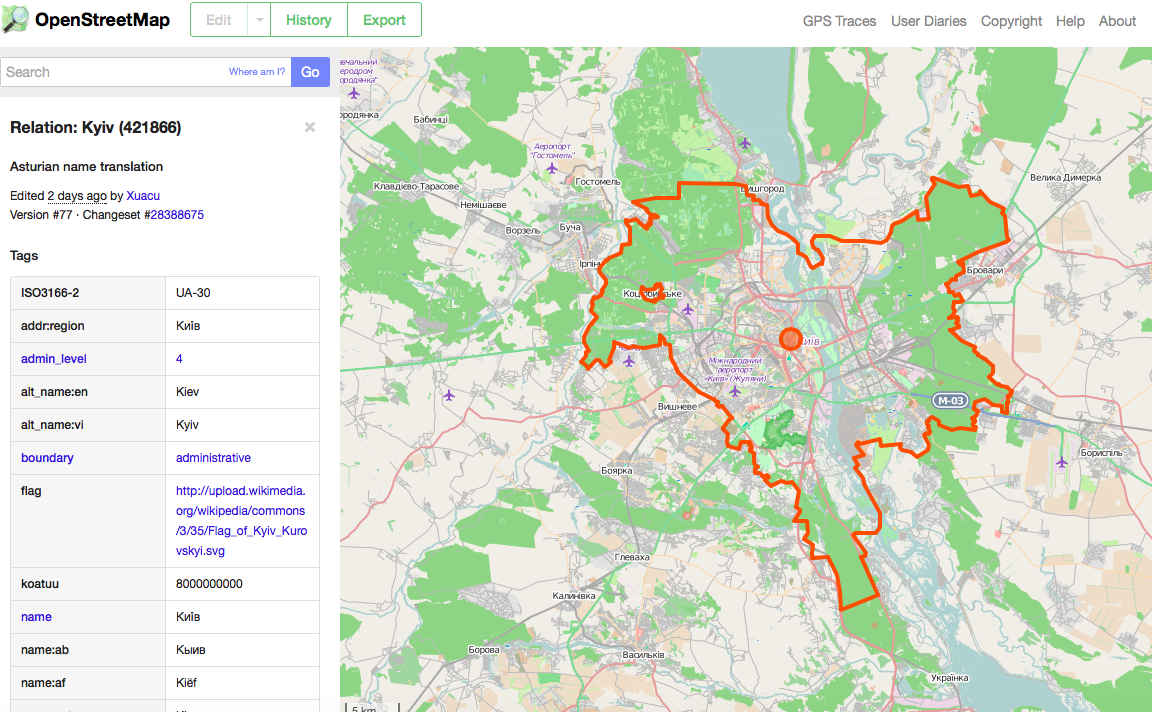
\includegraphics[scale=0.35]{keivinit.png}  
\par
I've done some zomming and choose next latitude and longitude parameters in my case:
\begin{itemize}
\item minimum latitude = 29.9048;
\item maximum latitude = 50.0986;
\item minimum longitude = 31.1600;
\item maximum longitude = 50.7052.
\end{itemize}
 
 Next step is to download my dataset. I've gone in \url{http://overpass-api.de/query_form.html}, where i can past some queries to download data what i need.\par

 My query is next:
 \begin{lstlisting}
(node(29.9048, 50.0986, 31.1600, 50.7052);<;);out;
\end{lstlisting}
Anyway there is exists numbers of variants loading data. One of them is simply go to this url \url{ http://overpass-api.de/api/map?bbox=29.9048,50.0986,31.1600,50.7052}. The xml file which I've already downloaded is very big, near 250mb. In my usual work i've chance working with xml, and files near 1mb is very hard to analyze. Let's move to processing this dataset.

\section*{Process Dataset}

As very first step, let's check what tags are in our dataset. Also would be helpful to check for attributes. Let's start from tags. 

\begin{lstlisting}[language=json,firstnumber=1]
{'bounds': 1,
 'member': 75124,
 'meta': 1,
 'nd': 1316743,
 'node': 1079619,
 'note': 1,
 'osm': 1,
 'relation': 5016,
 'tag': 417122,
 'way': 153102}
\end{lstlisting}
Next json is corresponded to tag attributes.
\begin{lstlisting}[language=json,firstnumber=1]
{'changeset': 1237737,
 'generator': 1,
 'id': 1237737,
 'k': 417122,
 'lat': 1079619,
 'lon': 1079619,
 'maxlat': 1,
 'maxlon': 1,
 'minlat': 1,
 'minlon': 1,
 'osm_base': 1,
 'ref': 1391867,
 'role': 75124,
 'timestamp': 1237737,
 'type': 75124,
 'uid': 1237737,
 'user': 1237737,
 'v': 417122,
 'version': 1237738}
\end{lstlisting}
First of all i would like to notice, that 'k' is key and 'v' is value. There are equal number of keys and values what is obvious. But it isn't clear what this keys are holding. I would like to explore more details and understand what keys and values have the most frequency in my dataset. In my opinion top 10 would be perfect for start.
\begin{lstlisting}[language=json,firstnumber=1]
{('surface', 9780),
 ('amenity', 9919),
 ('name:en', 10396),
 ('name:uk', 10646),
 ('name:ru', 12823),
 ('addr:street', 14084),
 ('name', 23862),
 ('addr:housenumber', 30646),
 ('highway', 67770),
 ('building', 73142)}
\end{lstlisting}
\end{document}